\documentclass[titlepage]{jsarticle}
\usepackage[dvipdfmx]{graphicx}
\usepackage{biblatex}
\usepackage[top=30truemm, left=20truemm,right=20truemm]{geometry}

\pagestyle{empty}

\begin{document}
\begin{figure}[h]
  \begin{minipage}{0.495\hsize}
    以下のように変数、定数を定義する。
      \begin{itemize}
        \item ミッションギア1速、5速の減速比: $r_1$, $r_5$
        \item ファイナルギアの減速比: $r_f = 4.785$
        \item エンジンの回転数: $n = 6200$ [rpm]
        \item エンジンのトルク: $T = 19$ [kgf $\cdot$ m]
        \item 自動車の最高速度: $v_{max} = 180$ [km/h]
        \item 自動車の最大登板角度: $\theta_{max} = 46^\circ$
        \item タイヤの直径: $d = 600$ [mm]
        \item 自動車の総重量: $m = 1360$ [kg]
        \item 重力加速度: $g$
      \end{itemize}
  \end{minipage}
  \begin{minipage}{0.495\hsize}
    \centering
    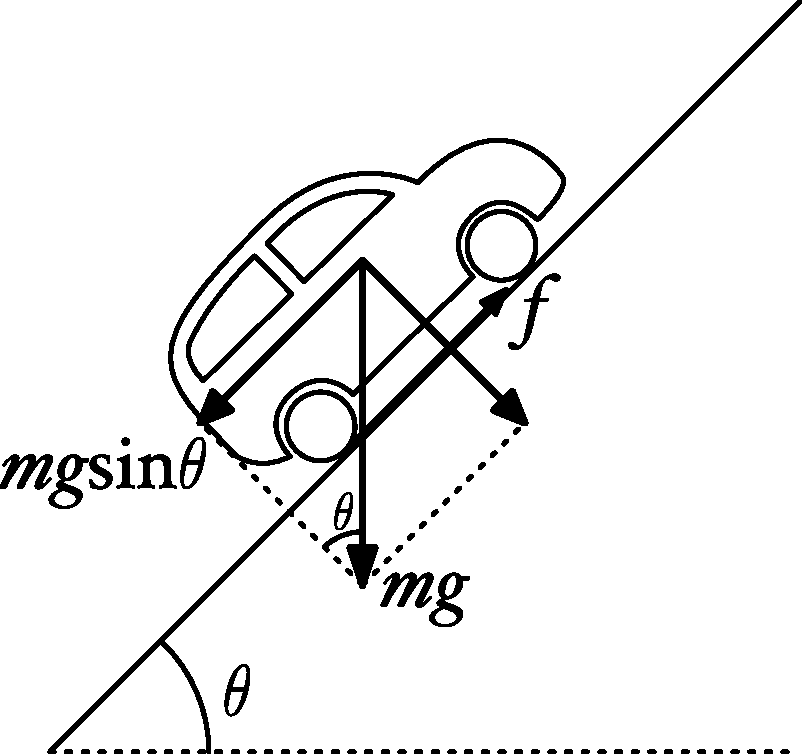
\includegraphics[width=6cm]{car.pdf}
  \end{minipage}
\end{figure}

まず、計算しやすいように各定数の単位を変換する。
\begin{eqnarray*}
  T &=& 19 \ [\mathrm{kgf \cdot m}] = 19g \ [\mathrm{N \cdot m}] \\
  v_{max} &=& 180 \ [\mathrm{km/h}] = 3000 \ [\mathrm{m/min}] \\
  d &=& 600 \ [\mathrm{mm}] = 0.6 \ [\mathrm m]
\end{eqnarray*}

$r_5$を求める。ミッションギアを5速に入れている時に180 [km/h]の速さが出れば良いので、
\begin{eqnarray*}
  \pi d \cdot \frac{n}{r_5r_f} &=& v_{max} \\
  r_5 &=& \frac{\pi d}{v_{max}} \cdot \frac{n}{r_f} \\
  &=& \frac{\pi 0.6 \ [\mathrm{m/r}]}{3000 \ [\mathrm{m/min}]} \cdot \frac{6200 \ [\mathrm{rpm}]}{4.785} \\
  &\approx& 0.2591 \pi
\end{eqnarray*}
となる。
$\pi$ = 3.14とすると、$r_5 \approx 0.8137$。

次に、$r_1$を求める。タイヤと地面に生じる摩擦力を$f$とすると、
図より、$f$が自動車にかかる重力より大きければ良いので、
\begin{eqnarray*}
  f = \frac{T \cdot r_1r_f}{\frac{d}{2}} &\geq& mg\sin \theta_{max} \\
  r_1 &\geq& \frac{d}{2} \cdot \frac{mg\sin \theta_{max}}{T \cdot r_f} \\
  &=& \frac{0.6}{2} \ [\mathrm m] \cdot \frac{1360g \cdot \sin 46^\circ \ [\mathrm N]}{19g \cdot 4.785 \ [\mathrm{N \cdot m}]} \\
  &\approx& 3.228
\end{eqnarray*}
となり、$r_1 \approx 3.228$。
\end{document}
